% =============================================================================
% uPyCore architecture diagrams -- system and subsystem figures for the paper
% =============================================================================
% Build (from this directory):
%   pdflatex upycore_architecture.tex && pdflatex upycore_architecture.tex
% Requires: article, tikz, booktabs, hyperref, geometry, microtype
%
% Every figure uses RTL / tool names (mpy_core, u_gc, G_SWEEP, ...) so it stays
% a faithful companion to upycore/rtl and upycore/docs. Where a block exists in
% the tree but is not yet wired into mpy_soc, the figure says so.
%
% Figures are laid out on an explicit centimetre grid (\B places a box by its
% centre), so they do not depend on relative-positioning heuristics.
% =============================================================================
\documentclass[11pt,a4paper]{article}

\usepackage[margin=0.9in]{geometry}
\usepackage{microtype}
\usepackage{booktabs}
\usepackage{xcolor}
\usepackage{hyperref}
\usepackage{caption}
\usepackage{float}
\usepackage{tikz}
\usetikzlibrary{arrows.meta,calc,shapes.geometric,shapes.misc,patterns}

\hypersetup{colorlinks=true, linkcolor=black, urlcolor=blue!50!black}
\captionsetup{font=small, labelfont=bf}
\setlength{\emergencystretch}{3em}

% ---- palette ---------------------------------------------------------------
\definecolor{cHost}{HTML}{E8EEF7}   % host-side tooling / pointers
\definecolor{cHW}{HTML}{FFF1D6}     % RTL blocks
\definecolor{cFW}{HTML}{E3F3E3}     % firmware / software / immediates
\definecolor{cMem}{HTML}{F0E6F6}    % storage
\definecolor{cWarn}{HTML}{F9DADA}   % not yet wired / failure
\definecolor{cLine}{HTML}{3A3A3A}

% ---- shared styles ---------------------------------------------------------
\tikzset{
  >={Stealth[length=2.2mm]},
  blk/.style={draw=cLine, rounded corners=2pt, thick, align=center,
              minimum height=8mm, inner sep=3pt, font=\small},
  host/.style={blk, fill=cHost},
  hw/.style={blk, fill=cHW},
  fw/.style={blk, fill=cFW},
  mem/.style={blk, fill=cMem},
  plain/.style={blk, fill=white},
  todo/.style={blk, fill=cWarn, dashed},
  dec/.style={diamond, aspect=2.4, draw=cLine, thick, fill=white, align=center,
              inner sep=0pt, font=\scriptsize},
  cond/.style={chamfered rectangle, chamfered rectangle xsep=4mm,
               chamfered rectangle ysep=0pt, draw=cLine, thick, fill=white,
               align=center, inner sep=3pt, font=\scriptsize},
  bus/.style={->, thick, cLine},
  bbus/.style={<->, thick, cLine},
  dbus/.style={->, thick, cLine, dashed},
  line/.style={thick, cLine},
  note/.style={font=\scriptsize\itshape, text=cLine!85, align=center},
  sig/.style={font=\scriptsize\ttfamily, fill=white, inner sep=1pt},
  lab/.style={font=\scriptsize\itshape, fill=white, inner sep=1pt},
  st/.style={circle, draw=cLine, thick, fill=cHW, minimum size=15mm,
             inner sep=0pt, font=\scriptsize\ttfamily, align=center},
}

\newcommand{\rtl}[1]{\texttt{\detokenize{#1}}}
\newcommand{\rtlx}[1]{\texttt{\expandafter\detokenize\expandafter{#1}}}
% \B{style}{width}{height}{name}{x,y}{text}   (centimetres, centred)
\newcommand{\B}[6]{\node[#1, minimum width=#2cm, minimum height=#3cm] (#4) at (#5) {#6};}

\title{uPyCore: System and Subsystem Diagrams\\
\large A microcontroller-class CPU whose instruction set is MicroPython bytecode}
\author{uPyCore systems notes\\
\rtl{docs/paper/systems/upycore_architecture.tex}}
\date{\today}

\begin{document}
\maketitle

\begin{abstract}
uPyCore executes MicroPython~v1.29.0 bytecode directly in hardware. Programs are
MicroPython source; the host \rtl{mpy-cross} compiler produces \rtl{.mpy}, a
linker packs firmware and program into one flash image, and a Verilator model
of \rtl{mpy_soc} runs it. There is no on-device compiler. This note collects the
figures for the paper: the end-to-end flow, the SoC, the core and its
firmware-hook split, the memory system and value encoding, the arithmetic
datapath, the garbage collector, and the interrupt/peripheral block.
Figures mark blocks that exist in the tree but are not yet wired into
\rtl{mpy_soc}. Colour key: \colorbox{cHW}{RTL}\ \colorbox{cFW}{firmware /
immediate}\ \colorbox{cHost}{host tooling / pointer}\ \colorbox{cMem}{storage}\
\colorbox{cWarn}{not yet wired / failure}.
\end{abstract}

\tableofcontents

% =============================================================================
\section{System overview}
% =============================================================================

Figure~\ref{fig:flow} shows the path from source to result. The unix oracle
(MicroPython built as the \rtl{upycore} variant) produces the golden output the
simulated hardware must match byte for byte; a second, independent compiler
(\rtl{vendor/upy2}, \rtl{mpyc}) is run through the same suite and byte-compared
with \rtl{mpy-cross}.

\begin{figure}[!htbp]
\centering
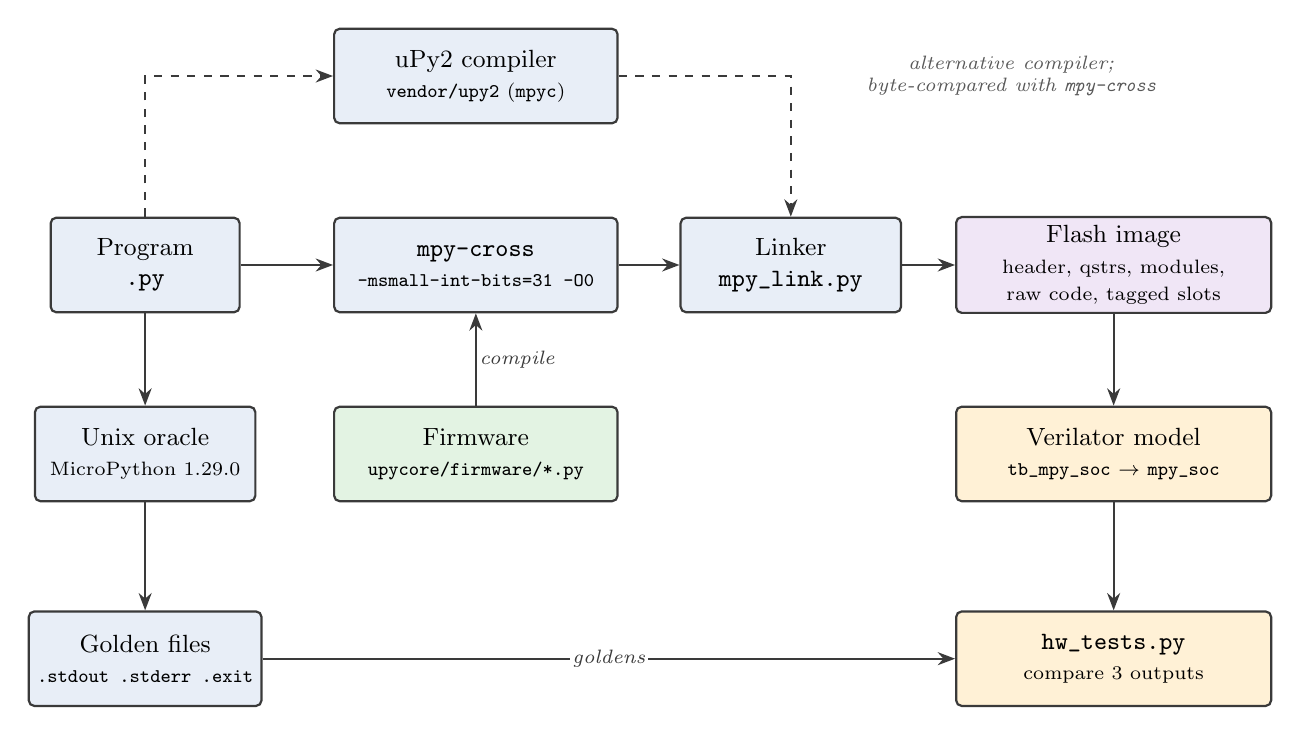
\begin{tikzpicture}
  \B{host}{2.4}{1.2}{src}{1.4,6}{Program\\\rtl{.py}}
  \B{host}{3.6}{1.2}{mpycross}{5.6,6}{\rtl{mpy-cross}\\\scriptsize\rtl{-msmall-int-bits=31 -O0}}
  \B{host}{2.8}{1.2}{link}{9.6,6}{Linker\\\rtl{mpy_link.py}}
  \B{mem}{4.0}{1.2}{img}{13.7,6}{Flash image\\\scriptsize header, qstrs, modules,\\[-1pt]\scriptsize raw code, tagged slots}

  \B{host}{3.6}{1.2}{upy2}{5.6,8.4}{uPy2 compiler\\\scriptsize\rtl{vendor/upy2} (\rtl{mpyc})}
  \B{fw}{3.6}{1.2}{fw}{5.6,3.6}{Firmware\\\scriptsize\rtl{upycore/firmware/*.py}}

  \B{host}{2.8}{1.2}{oracle}{1.4,3.6}{Unix oracle\\\scriptsize MicroPython 1.29.0}
  \B{host}{2.8}{1.2}{gold}{1.4,1.0}{Golden files\\\scriptsize\rtl{.stdout .stderr .exit}}

  \B{hw}{4.0}{1.2}{sim}{13.7,3.6}{Verilator model\\\scriptsize\rtl{tb_mpy_soc} $\to$ \rtl{mpy_soc}}
  \B{hw}{4.0}{1.2}{cmp}{13.7,1.0}{\rtl{hw_tests.py}\\\scriptsize compare 3 outputs}

  \draw[bus] (src) -- (mpycross);
  \draw[bus] (mpycross) -- (link);
  \draw[bus] (link) -- (img);
  \draw[bus] (fw) -- node[lab, right] {compile} (mpycross);
  \draw[bus] (img) -- (sim);
  \draw[bus] (sim) -- (cmp);
  \draw[bus] (src.south) -- (oracle.north);
  \draw[bus] (oracle) -- (gold);
  \draw[bus] (gold) -- node[lab] {goldens} (cmp);

  % uPy2 alternative path
  \draw[dbus] (src.north) |- (upy2.west);
  \draw[dbus] (upy2.east) -| (link.north);
  \node[note] at (12.4,8.4) {alternative compiler;\\byte-compared with \rtl{mpy-cross}};
\end{tikzpicture}
\caption{Build and verification flow. Solid arrows are the default
\rtl{make test} path; dashed arrows are the uPy2 compiler pass
(\rtl{make test-compiler}).}
\label{fig:flow}
\end{figure}

% -----------------------------------------------------------------------------
\section{SoC structure}
% -----------------------------------------------------------------------------

\rtl{mpy_soc} instantiates exactly three blocks---\rtl{mpy_core}, \rtl{mpy_gc},
and \rtl{mpy_mem}---on a single memory port. The collector owns the port while
\rtl{g_busy} is high; the core only waits during an allocation or collection,
so the two never contend. Accesses to the simulator-control page are answered
inside the SoC and never reach memory.

\begin{figure}[!htbp]
\centering
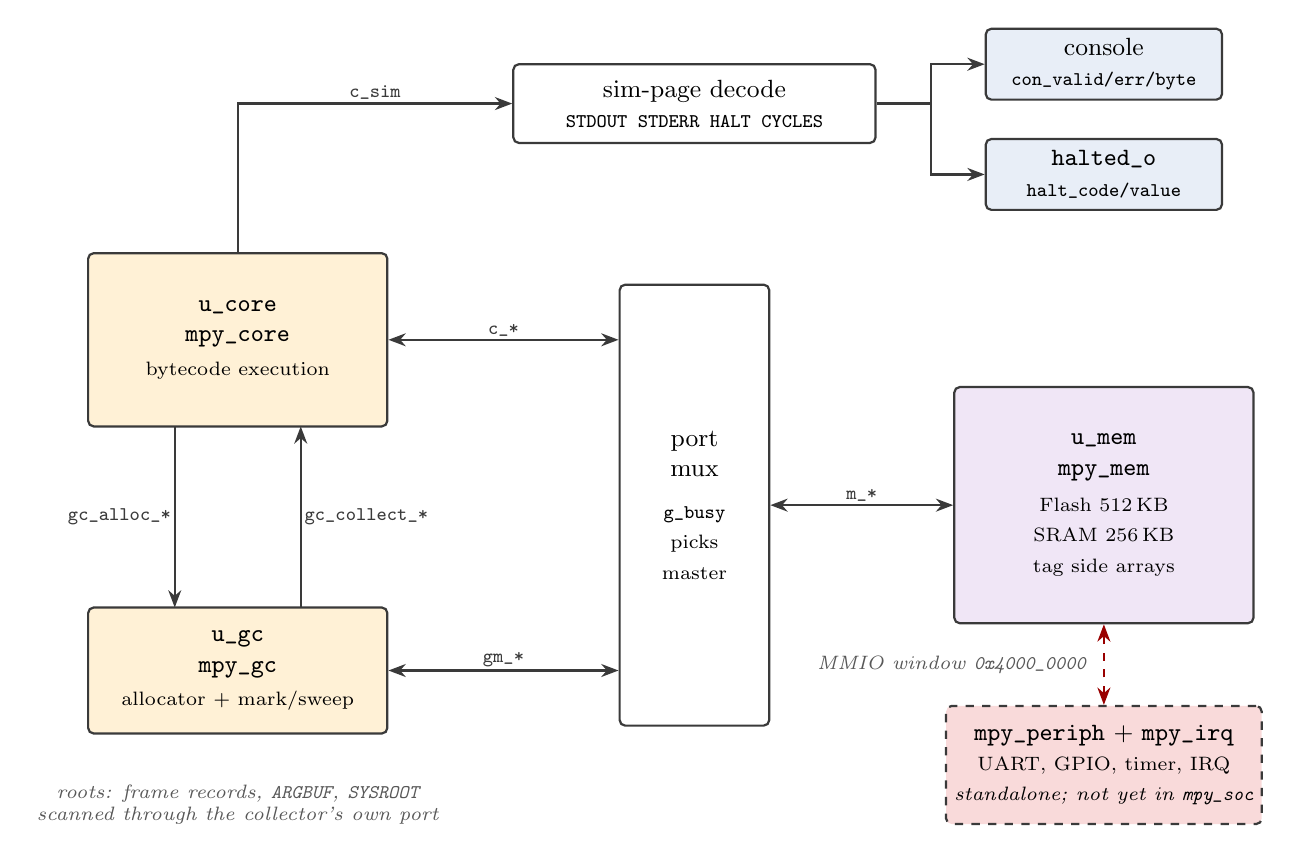
\begin{tikzpicture}
  \B{hw}{3.8}{2.2}{core}{2.2,5.6}{\textbf{\rtl{u_core}}\\\rtl{mpy_core}\\[1pt]\scriptsize bytecode execution}
  \B{hw}{3.8}{1.6}{gc}{2.2,1.4}{\textbf{\rtl{u_gc}}\\\rtl{mpy_gc}\\[1pt]\scriptsize allocator + mark/sweep}
  \B{plain}{1.9}{5.6}{mux}{8.0,3.5}{port\\mux\\[4pt]\scriptsize\rtl{g_busy}\\\scriptsize picks\\\scriptsize master}
  \B{mem}{3.8}{3.0}{mem}{13.2,3.5}{\textbf{\rtl{u_mem}}\\\rtl{mpy_mem}\\[2pt]\scriptsize Flash 512\,KB\\\scriptsize SRAM 256\,KB\\\scriptsize tag side arrays}

  \B{plain}{4.6}{1.0}{sim}{8.0,8.6}{sim-page decode\\\scriptsize\rtl{STDOUT STDERR HALT CYCLES}}
  \B{host}{3.0}{0.9}{con}{13.2,9.1}{console\\\scriptsize\rtl{con_valid/err/byte}}
  \B{host}{3.0}{0.9}{halt}{13.2,7.7}{\rtl{halted_o}\\\scriptsize\rtl{halt_code/value}}
  \B{todo}{3.8}{1.5}{periph}{13.2,0.2}{\rtl{mpy_periph} + \rtl{mpy_irq}\\\scriptsize UART, GPIO, timer, IRQ\\\scriptsize\itshape standalone; not yet in \rtl{mpy_soc}}

  \draw[bbus] (core.east) -- node[sig, above] {\rtl{c_*}} (mux.west |- core.east);
  \draw[bbus] (gc.east) -- node[sig, above] {\rtl{gm_*}} (mux.west |- gc.east);
  \draw[bbus] (mux.east) -- node[sig, above] {\rtl{m_*}} (mem.west);

  \draw[bus] (core.north) -- (2.2,8.6) -- node[sig, above] {\rtl{c_sim}} (sim.west);
  \draw[bus] (sim.east) -- (11.0,8.6) |- (con.west);
  \draw[bus] (11.0,8.6) |- (halt.west);

  \draw[bus] (1.4,4.5) -- node[sig, left] {\rtl{gc_alloc_*}} (1.4,2.2);
  \draw[bus] (3.0,2.2) -- node[sig, right] {\rtl{gc_collect_*}} (3.0,4.5);
  \node[note] at (2.2,-0.3) {roots: frame records, \rtl{ARGBUF}, \rtl{SYSROOT}\\scanned through the collector's own port};

  \draw[bbus, dashed, red!60!black] (periph.north) -- node[note, left, xshift=-1mm] {MMIO window \rtl{0x4000_0000}} (mem.south);
\end{tikzpicture}
\caption{\rtl{mpy_soc}. Solid blocks are instantiated; the dashed red block has
RTL and a testbench but is not yet connected.}
\label{fig:soc}
\end{figure}

\begin{table}[!htbp]
\centering
\caption{Top-level observability exported by \rtl{mpy_soc}.}
\begin{tabular}{@{}ll@{}}
\toprule
Port group & Meaning \\
\midrule
\rtl{con_valid_o con_err_o con_byte_o} & one console byte per pulse, stdout or stderr \\
\rtl{halted_o halt_code_o halt_value_o} & core halt or \rtl{SIM_HALT} store (\rtl{ABI_HALT_SYSEXIT}) \\
\rtl{cycles_o ops_o} & cycle and retired-opcode counters \\
\rtl{gc_collections_o gc_free_o} & collector statistics \\
\rtl{trace_*} & per-opcode trace: PC, opcode byte, stack pointer \\
\bottomrule
\end{tabular}
\end{table}

% =============================================================================
\section{The execution core}
% =============================================================================

The core keeps \emph{one frame live in registers}. It executes the common shape
of every opcode itself and delegates the rest to \emph{firmware hooks}:
MicroPython functions in flash that the core calls like any Python function.
Figure~\ref{fig:core} gives the structure; Figure~\ref{fig:hook} gives the
dispatch decision.

\begin{figure}[!htbp]
\centering
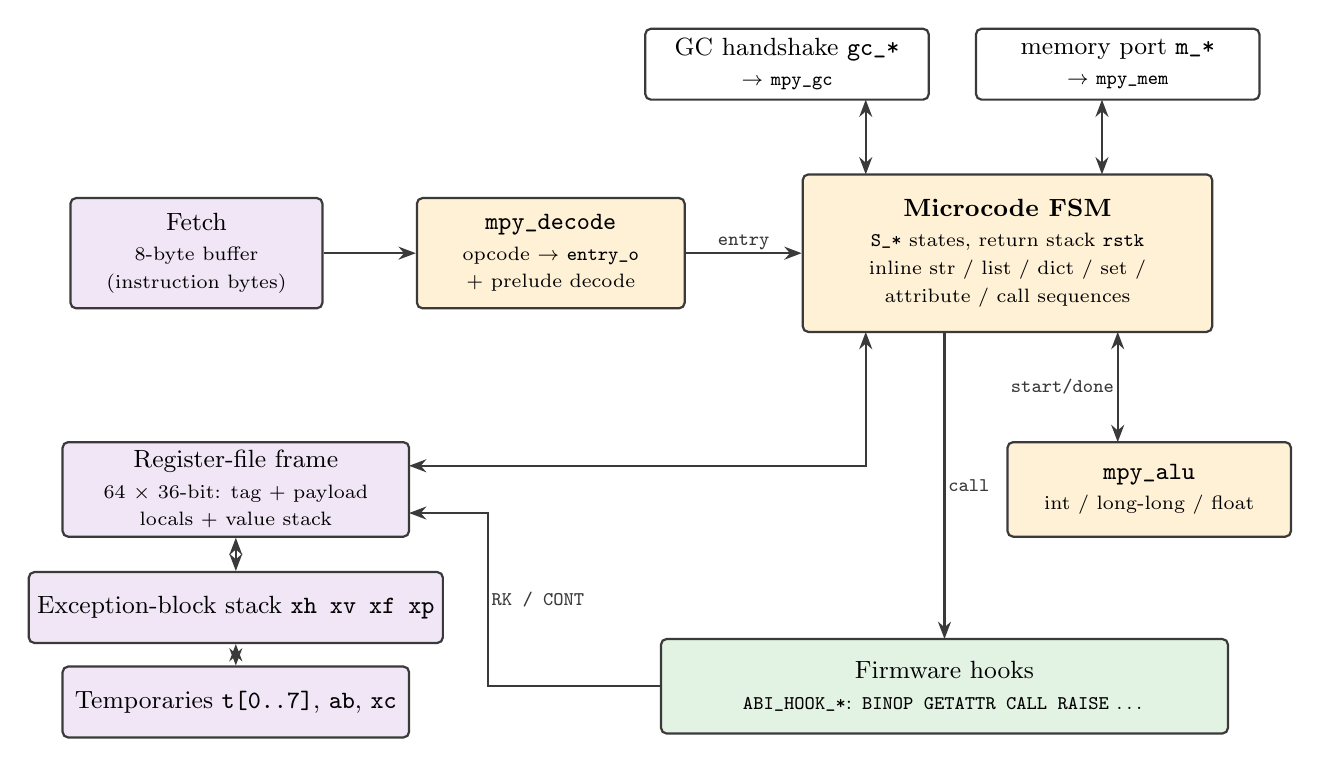
\begin{tikzpicture}
  \B{plain}{3.6}{0.9}{gcport}{9.4,8.8}{GC handshake \rtl{gc_*}\\\scriptsize $\to$ \rtl{mpy_gc}}
  \B{plain}{3.6}{0.9}{mport}{13.6,8.8}{memory port \rtl{m_*}\\\scriptsize $\to$ \rtl{mpy_mem}}

  \B{mem}{3.2}{1.4}{fetch}{1.9,6.4}{Fetch\\\scriptsize 8-byte buffer\\[-1pt]\scriptsize (instruction bytes)}
  \B{hw}{3.4}{1.4}{dec}{6.4,6.4}{\rtl{mpy_decode}\\\scriptsize opcode $\to$ \rtl{entry_o}\\[-1pt]\scriptsize + prelude decode}
  \B{hw}{5.2}{2.0}{fsm}{12.2,6.4}{\textbf{Microcode FSM}\\\scriptsize \rtl{S_*} states, return stack \rtl{rstk}\\[-1pt]\scriptsize inline str / list / dict / set /\\[-1pt]\scriptsize attribute / call sequences}

  \B{mem}{4.4}{1.2}{rf}{2.4,3.4}{Register-file frame\\\scriptsize 64 $\times$ 36-bit: tag + payload\\[-1pt]\scriptsize locals + value stack}
  \B{mem}{4.4}{0.9}{xs}{2.4,1.9}{Exception-block stack \rtl{xh xv xf xp}}
  \B{mem}{4.4}{0.9}{tmp}{2.4,0.7}{Temporaries \rtl{t[0..7]}, \rtl{ab}, \rtl{xc}}

  \B{hw}{3.6}{1.2}{alu}{14.0,3.4}{\rtl{mpy_alu}\\\scriptsize int / long-long / float}
  \B{fw}{7.2}{1.2}{hooks}{11.4,0.9}{Firmware hooks\\\scriptsize\rtl{ABI_HOOK_*}: \rtl{BINOP GETATTR CALL RAISE} \dots}

  \draw[bus] (fetch) -- (dec);
  \draw[bus] (dec) -- node[sig, above] {\rtl{entry}} (fsm);
  \draw[bbus] (10.4,7.4) -- (10.4,8.35);
  \draw[bbus] (13.4,7.4) -- (13.4,8.35);
  \draw[bbus] (rf) -- (xs);
  \draw[bbus] (xs) -- (tmp);

  \draw[bbus] (4.6,3.7) -- (10.4,3.7) -- (10.4,5.4);
  \draw[bbus] (13.6,5.4) -- node[sig, left] {\rtl{start/done}} (13.6,4.0);

  \draw[bus] (11.4,5.4) -- node[sig, right] {call} (11.4,1.5);
  \draw[bus] (hooks.west) -- (5.6,0.9) -- node[sig, right] {\rtl{RK / CONT}} (5.6,3.1) -- (4.6,3.1);
\end{tikzpicture}
\caption{\rtl{mpy_core}. The microcode FSM sequences each opcode; instruction
fetch and decode, the register frame, the ALU, and the two external handshakes
are the only structural blocks. A hook returns through a return kind
(\rtl{RK}) or continuation (\rtl{CONT}).}
\label{fig:core}
\end{figure}

\begin{figure}[!htbp]
\centering
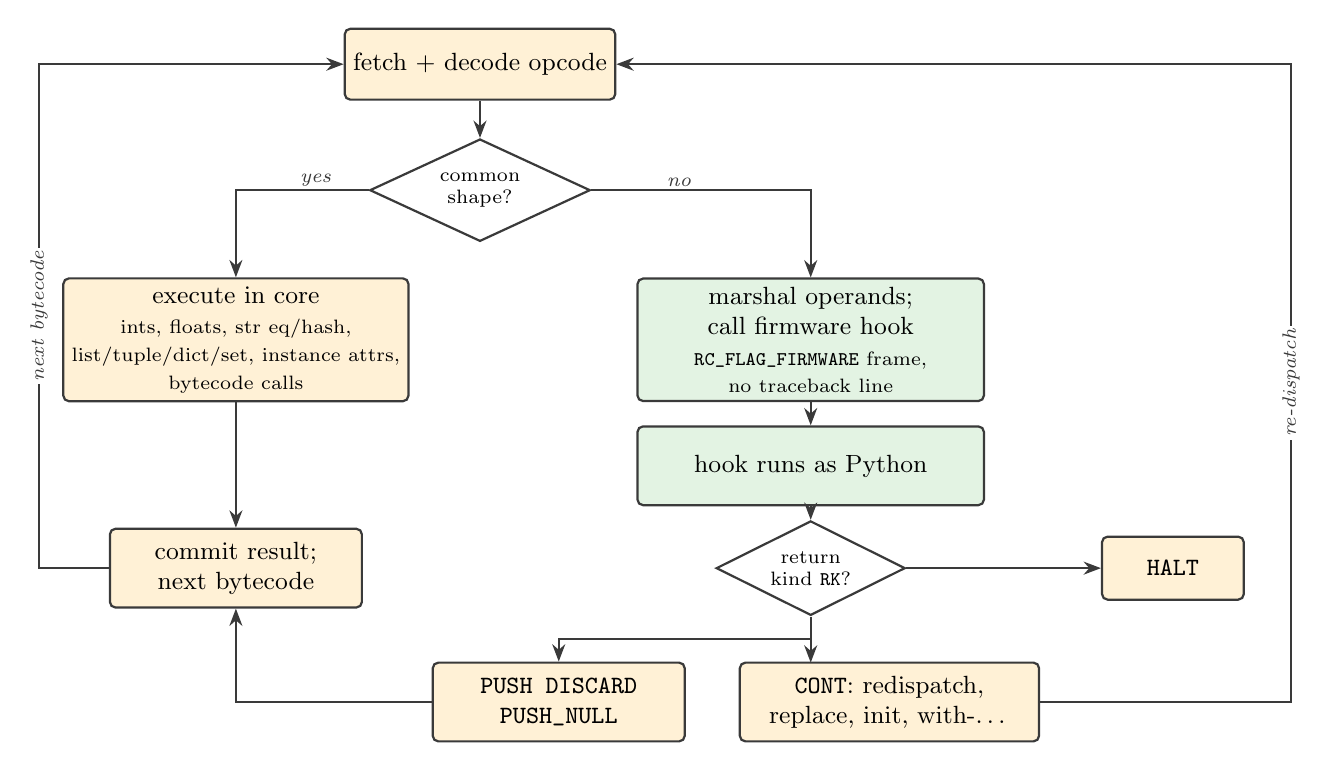
\begin{tikzpicture}
  \B{hw}{3.4}{0.9}{fetch}{5.0,8.5}{fetch + decode opcode}
  \node[dec, minimum width=2.8cm, minimum height=1.3cm] (common) at (5.0,6.9) {common\\shape?};
  \B{hw}{4.2}{1.5}{native}{1.9,5.0}{execute in core\\\scriptsize ints, floats, str eq/hash,\\[-1pt]\scriptsize list/tuple/dict/set, instance attrs,\\[-1pt]\scriptsize bytecode calls}
  \B{fw}{4.4}{1.5}{hook}{9.2,5.0}{marshal operands;\\call firmware hook\\\scriptsize\rtl{RC_FLAG_FIRMWARE} frame,\\[-1pt]\scriptsize no traceback line}
  \B{fw}{4.4}{1.0}{run}{9.2,3.4}{hook runs as Python}
  \node[dec, minimum width=2.4cm, minimum height=1.2cm] (rk) at (9.2,2.1) {return\\kind \rtl{RK}?};
  \B{hw}{3.2}{1.0}{commit}{1.9,2.1}{commit result;\\next bytecode}
  \B{hw}{3.2}{1.0}{push}{6.0,0.4}{\rtl{PUSH DISCARD}\\\rtl{PUSH_NULL}}
  \B{hw}{3.8}{1.0}{cont}{10.2,0.4}{\rtl{CONT}: redispatch,\\replace, init, with-\dots}
  \B{hw}{1.8}{0.8}{halt}{13.8,2.1}{\rtl{HALT}}

  \draw[bus] (fetch) -- (common);
  \draw[bus] (common.west) -| node[lab, pos=0.2, above] {yes} (native);
  \draw[bus] (common.east) -| node[lab, pos=0.2, above] {no} (hook);
  \draw[bus] (hook) -- (run);
  \draw[bus] (run) -- (rk);
  \draw[bus] (native) -- (commit);
  \draw[bus] (rk.south) -- (9.2,1.2) -| (push.north);
  \draw[bus] (9.2,1.2) -- (9.2,0.9);
  \draw[bus] (rk.east) -- (halt.west);
  \draw[bus] (push.west) -| (commit.south);
  \draw[bus] (commit.west) -- (-0.6,2.1) -- node[lab, rotate=90] {next bytecode} (-0.6,8.5) -- (fetch.west);
  \draw[bus] (cont.east) -- (15.3,0.4) -- node[lab, rotate=90] {re-dispatch} (15.3,8.5) -- (fetch.east);
\end{tikzpicture}
\caption{Opcode dispatch. A hook returns through a return kind \rtl{RK}; a
continuation \rtl{CONT} (\rtl{REDISPATCH}, \rtl{REPLACE}, \rtl{INIT}, the
\rtl{WITH_*} family) lets a hook finish by re-running the original opcode.}
\label{fig:hook}
\end{figure}

\subsection{Call and return}

A call spills the caller's whole frame to a 512-byte record in SRAM and builds
the callee's record above it; a return or unwinding exception refills the
caller. Thirty-two records fit the reserve; a 33rd faults and software reports
\rtl{RuntimeError: maximum recursion depth exceeded}.

\begin{figure}[!htbp]
\centering
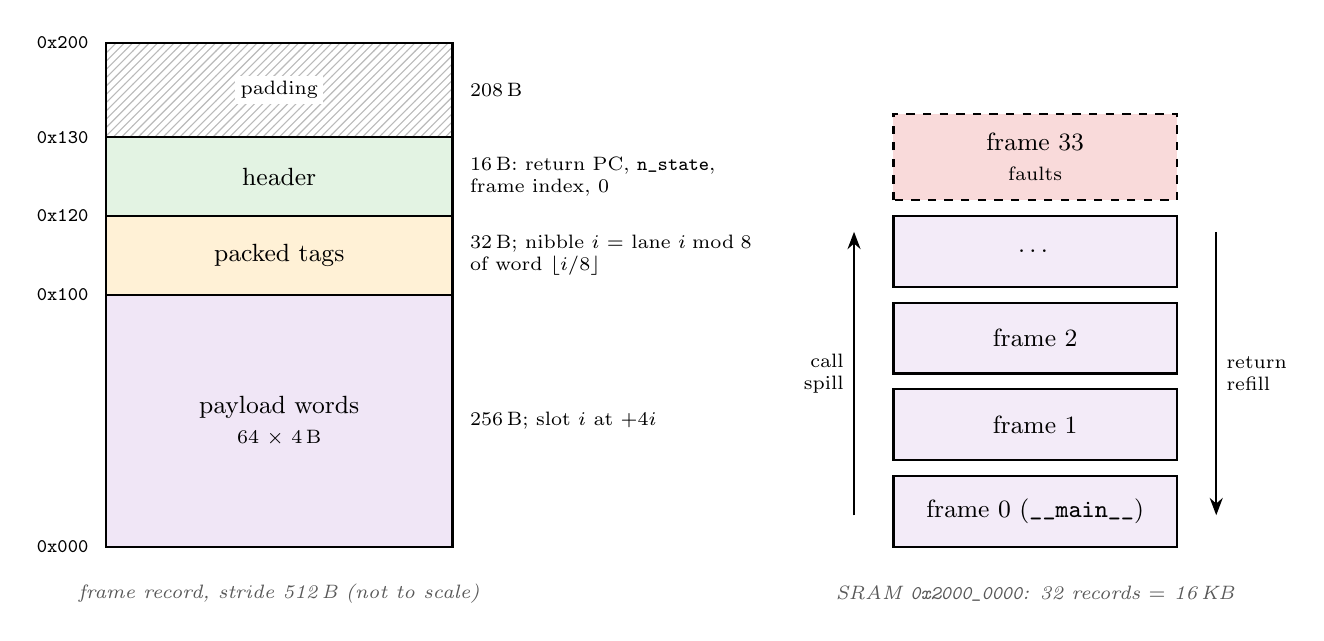
\begin{tikzpicture}
  % one frame record (not to scale)
  \draw[thick,fill=cMem]  (0,0)   rectangle (4.4,3.2) node[midway,align=center,font=\small] {payload words\\\scriptsize 64 $\times$ 4\,B};
  \draw[thick,fill=cHW]   (0,3.2) rectangle (4.4,4.2) node[midway,font=\small] {packed tags};
  \draw[thick,fill=cFW]   (0,4.2) rectangle (4.4,5.2) node[midway,font=\small] {header};
  \draw[thick,pattern=north east lines,pattern color=cLine!35] (0,5.2) rectangle (4.4,6.4);
  \node[fill=white,inner sep=2pt,font=\scriptsize] at (2.2,5.8) {padding};
  \foreach \y/\t in {0/0x000, 3.2/0x100, 4.2/0x120, 5.2/0x130, 6.4/0x200}
    \node[left,font=\scriptsize] at (-0.1,\y) {\rtlx{\t}};
  \node[right,font=\scriptsize,align=left] at (4.5,1.6) {256\,B; slot $i$ at $+4i$};
  \node[right,font=\scriptsize,align=left] at (4.5,3.7) {32\,B; nibble $i$ = lane $i \bmod 8$\\of word $\lfloor i/8\rfloor$};
  \node[right,font=\scriptsize,align=left] at (4.5,4.7) {16\,B: return PC, \rtl{n_state},\\frame index, 0};
  \node[right,font=\scriptsize,align=left] at (4.5,5.8) {208\,B};
  \node[note] at (2.2,-0.6) {frame record, stride 512\,B (not to scale)};

  % call stack
  \begin{scope}[xshift=10.0cm]
    \foreach \i/\lab in {0/{frame 0 (\rtl{__main__})},1/{frame 1},2/{frame 2},3/{\dots}}
      \draw[thick,fill=cMem!80] (0,\i*1.1) rectangle (3.6,\i*1.1+0.9) node[midway,font=\small] {\lab};
    \draw[thick,fill=cWarn,dashed] (0,4.4) rectangle (3.6,5.5) node[midway,font=\small,align=center] {frame 33\\\scriptsize faults};
    \draw[->,thick] (-0.5,0.4) -- node[left,font=\scriptsize,align=right] {call\\spill} (-0.5,4.0);
    \draw[->,thick] (4.1,4.0) -- node[right,font=\scriptsize,align=left] {return\\refill} (4.1,0.4);
    \node[note] at (1.8,-0.6) {SRAM \rtl{0x2000_0000}: 32 records $=$ 16\,KB};
  \end{scope}
\end{tikzpicture}
\caption{Frame record layout (left) and the 32-deep call stack in the SRAM
frame reserve (right). A spill writes every physical register; tags for these
slots live in the packed words of the record, not in a second copy.}
\label{fig:frame}
\end{figure}

% =============================================================================
\section{Memory system and value encoding}
% =============================================================================

There is no DRAM and no cache. SRAM is one cycle; flash adds
\rtl{MPY_FLASH_WAIT_STATES} (default~1). Every 32-bit data word has a 4-bit tag
held in a side array, eight tags to a word.

\begin{figure}[!htbp]
\centering
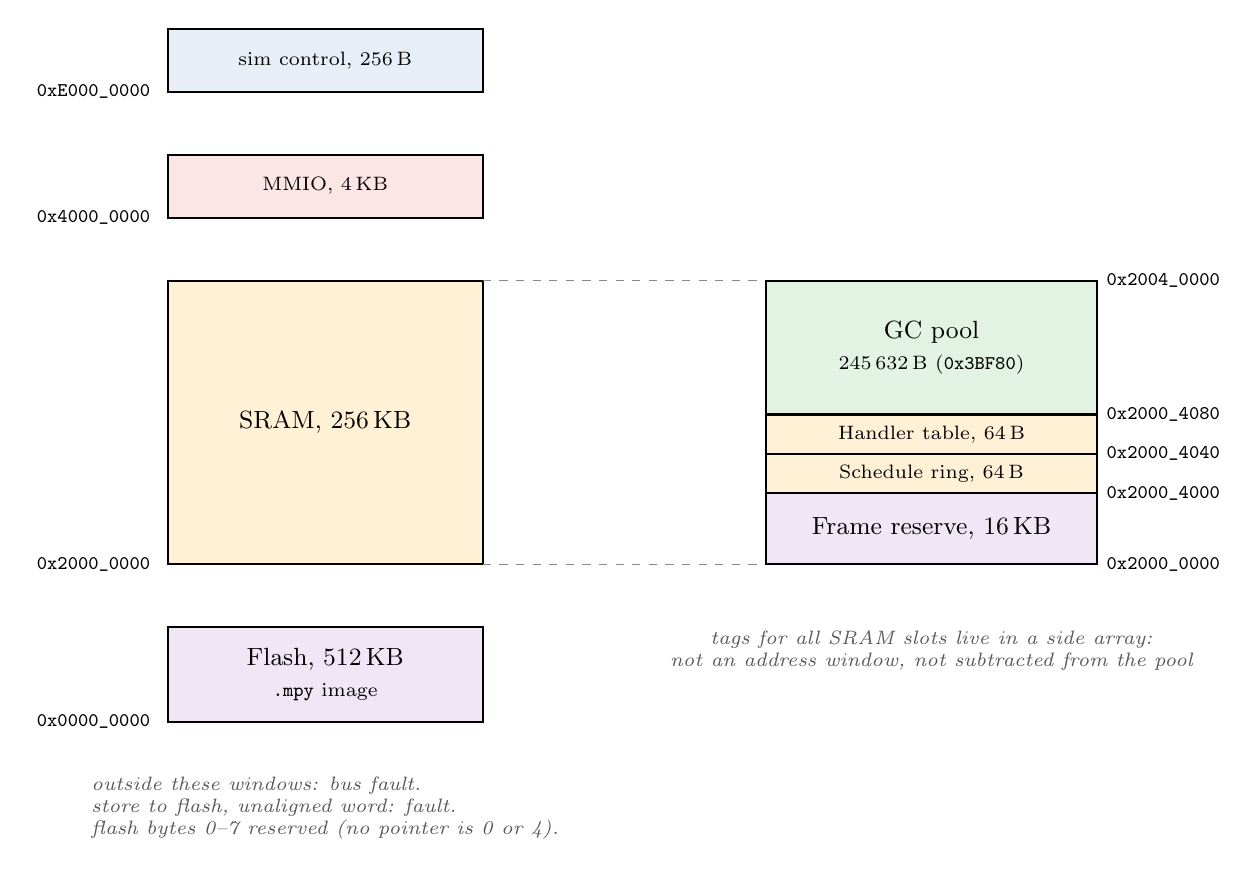
\begin{tikzpicture}
  % full address space (not to scale)
  \draw[thick,fill=cMem]  (0,0)   rectangle (4.0,1.2) node[midway,align=center,font=\small] {Flash, 512\,KB\\\scriptsize\rtl{.mpy} image};
  \draw[thick,fill=cHW]   (0,2.0) rectangle (4.0,5.6) node[midway,align=center,font=\small] {SRAM, 256\,KB};
  \draw[thick,fill=cWarn!70] (0,6.4) rectangle (4.0,7.2) node[midway,font=\scriptsize] {MMIO, 4\,KB};
  \draw[thick,fill=cHost] (0,8.0) rectangle (4.0,8.8) node[midway,font=\scriptsize] {sim control, 256\,B};
  \foreach \y/\t in {0/0x0000_0000, 2.0/0x2000_0000, 6.4/0x4000_0000, 8.0/0xE000_0000}
    \node[left,font=\scriptsize] at (-0.1,\y) {\rtlx{\t}};
  \node[note,align=left] at (2.0,-1.1) {outside these windows: bus fault.\\store to flash, unaligned word: fault.\\flash bytes 0--7 reserved (no pointer is 0 or 4).};

  % SRAM breakdown
  \draw[dashed,cLine!60] (4.0,2.0) -- (7.6,2.0);
  \draw[dashed,cLine!60] (4.0,5.6) -- (7.6,5.6);
  \begin{scope}[xshift=7.6cm]
    \draw[thick,fill=cMem] (0,2.0) rectangle (4.2,2.9) node[midway,font=\small] {Frame reserve, 16\,KB};
    \draw[thick,fill=cHW]  (0,2.9) rectangle (4.2,3.4) node[midway,font=\scriptsize] {Schedule ring, 64\,B};
    \draw[thick,fill=cHW]  (0,3.4) rectangle (4.2,3.9) node[midway,font=\scriptsize] {Handler table, 64\,B};
    \draw[thick,fill=cFW]  (0,3.9) rectangle (4.2,5.6) node[midway,align=center,font=\small] {GC pool\\\scriptsize 245\,632\,B (\rtl{0x3BF80})};
    \foreach \y/\t in {2.0/0x2000_0000, 2.9/0x2000_4000, 3.4/0x2000_4040, 3.9/0x2000_4080, 5.6/0x2004_0000}
      \node[right,font=\scriptsize] at (4.2,\y) {\rtlx{\t}};
    \node[note] at (2.1,0.9) {tags for all SRAM slots live in a side array:\\not an address window, not subtracted from the pool};
  \end{scope}
\end{tikzpicture}
\caption{Address map. The frame-reserve tags are the packed words inside each
frame record; the handler table is a GC root.}
\label{fig:map}
\end{figure}

\subsection{Tagged values}

A value is a 4-bit tag beside a 32-bit payload; the register file is a single
36-bit array. Figure~\ref{fig:tags} groups the sixteen tag codes by what the
payload means and whether the collector follows it.

\begin{figure}[!htbp]
\centering
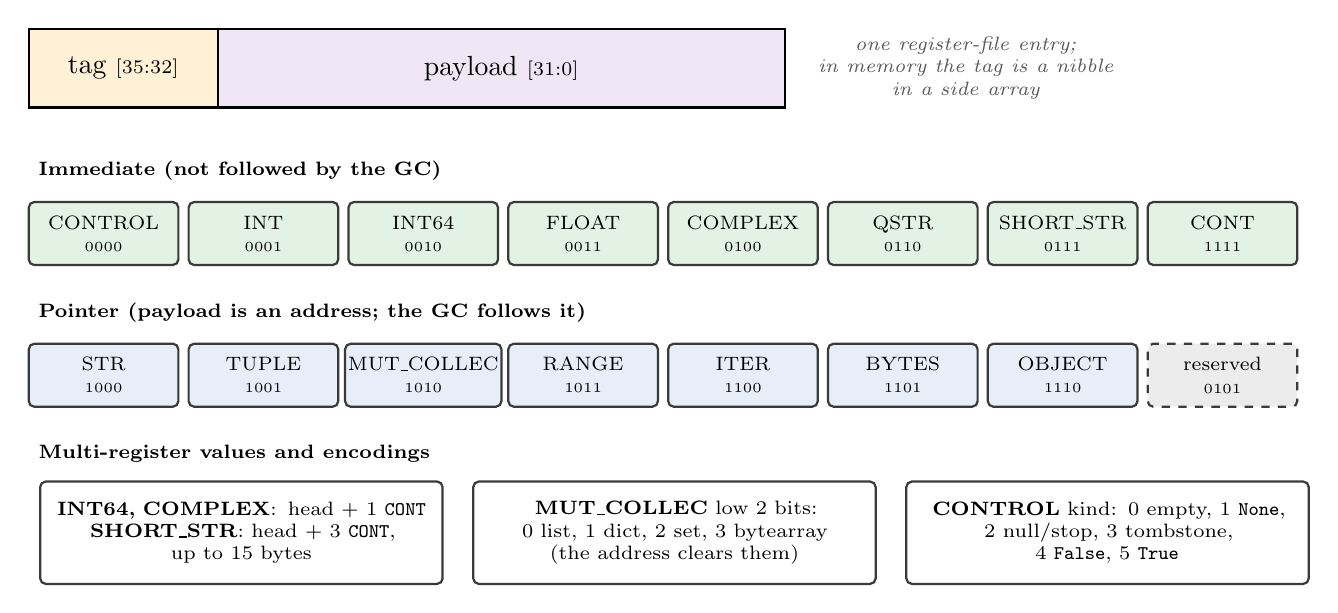
\begin{tikzpicture}
  \draw[thick,fill=cHW]   (0,8.2) rectangle (2.4,9.2) node[midway] {tag \scriptsize[35:32]};
  \draw[thick,fill=cMem]  (2.4,8.2) rectangle (9.6,9.2) node[midway] {payload \scriptsize[31:0]};
  \node[note,anchor=west] at (9.9,8.7) {one register-file entry;\\in memory the tag is a nibble\\in a side array};

  \node[font=\scriptsize\bfseries,anchor=west] at (0,7.4) {Immediate (not followed by the GC)};
  \foreach \i/\t in {0/{CONTROL\\\tiny0000},1/{INT\\\tiny0001},2/{INT64\\\tiny0010},3/{FLOAT\\\tiny0011},4/{COMPLEX\\\tiny0100},5/{QSTR\\\tiny0110},6/{SHORT\_STR\\\tiny0111},7/{CONT\\\tiny1111}}
    \node[blk,fill=cFW,minimum width=1.9cm,inner sep=1pt,font=\fontsize{7}{8}\selectfont] at (\i*2.03+0.95,6.6) {\t};

  \node[font=\scriptsize\bfseries,anchor=west] at (0,5.6) {Pointer (payload is an address; the GC follows it)};
  \foreach \i/\t in {0/{STR\\\tiny1000},1/{TUPLE\\\tiny1001},2/{MUT\_COLLEC\\\tiny1010},3/{RANGE\\\tiny1011},4/{ITER\\\tiny1100},5/{BYTES\\\tiny1101},6/{OBJECT\\\tiny1110}}
    \node[blk,fill=cHost,minimum width=1.9cm,inner sep=1pt,font=\fontsize{7}{8}\selectfont] at (\i*2.03+0.95,4.8) {\t};
  \node[blk,fill=gray!15,dashed,minimum width=1.9cm,inner sep=1pt,font=\fontsize{7}{8}\selectfont] at (7*2.03+0.95,4.8) {reserved\\\tiny0101};

  \node[font=\scriptsize\bfseries,anchor=west] at (0,3.8) {Multi-register values and encodings};
  \node[plain,font=\scriptsize,text width=4.9cm,minimum height=1.3cm] at (2.7,2.8) {\mbox{\textbf{INT64, COMPLEX}}: head + 1 \rtl{CONT}\\\textbf{SHORT\_STR}: head + 3 \rtl{CONT},\\up to 15 bytes};
  \node[plain,font=\scriptsize,text width=4.9cm,minimum height=1.3cm] at (8.2,2.8) {\textbf{MUT\_COLLEC} low 2 bits:\\0 list, 1 dict, 2 set, 3 bytearray\\(the address clears them)};
  \node[plain,font=\scriptsize,text width=4.9cm,minimum height=1.3cm] at (13.7,2.8) {\textbf{CONTROL} kind: 0 empty, 1 \rtl{None},\\2 null/stop, 3 tombstone,\\4 \rtl{False}, 5 \rtl{True}};
\end{tikzpicture}
\caption{Value encoding. \rtl{False} and \rtl{True} are \rtl{CONTROL} kinds~4
and~5 and double as integers 0 and~1 in arithmetic and hashing.}
\label{fig:tags}
\end{figure}

\subsection{Heap object layouts}

\begin{figure}[!htbp]
\centering
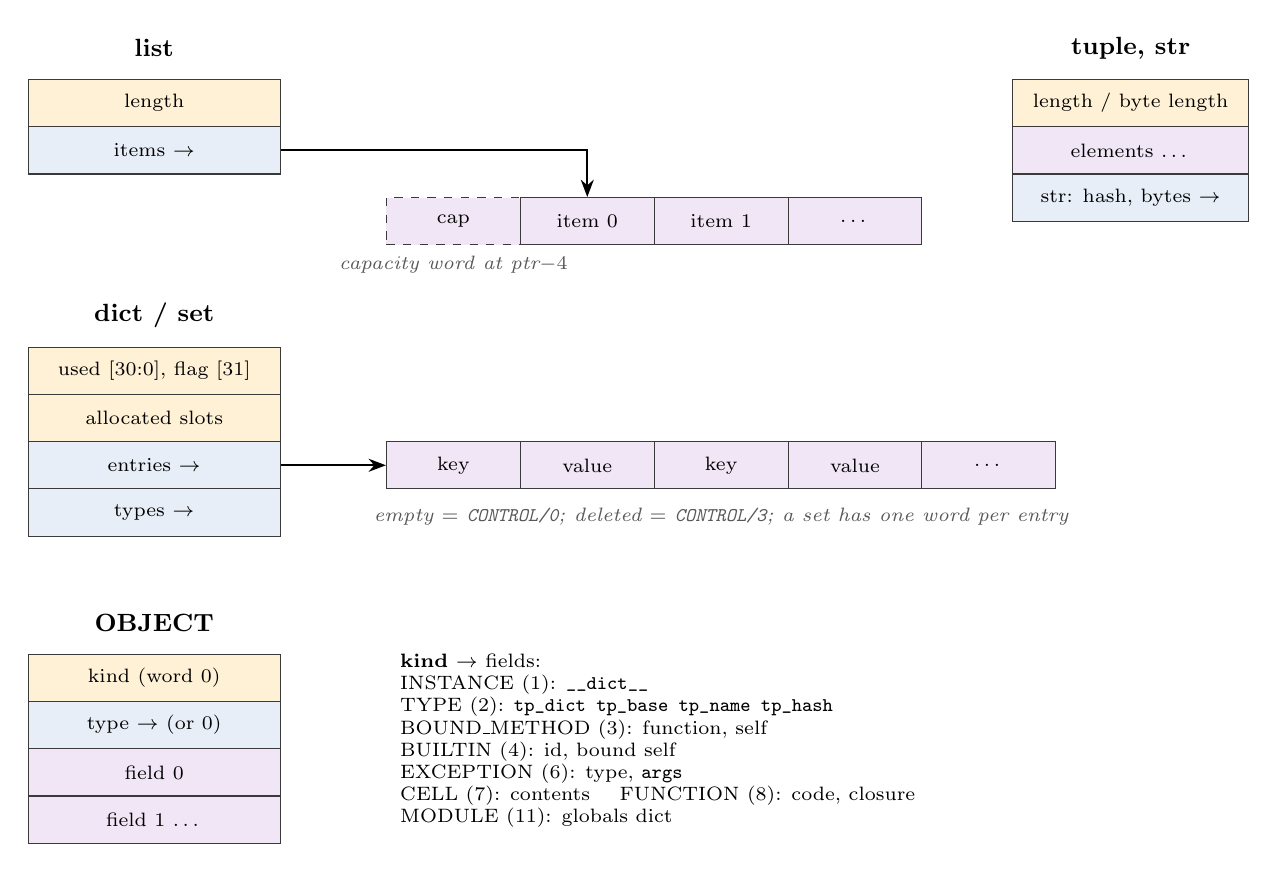
\begin{tikzpicture}[
  cell/.style={draw=cLine, minimum height=0.6cm, font=\scriptsize, inner sep=1pt, anchor=center},
  hdr/.style={cell, minimum width=3.2cm, fill=cHW},
  ptr/.style={cell, minimum width=3.2cm, fill=cHost},
  dat/.style={cell, minimum width=1.7cm, fill=cMem},
  ttl/.style={font=\small\bfseries}]

  % list ------------------------------------------------------------------
  \node[ttl] at (1.6,6.9) {list};
  \node[hdr] at (1.6,6.2) {length};
  \node[ptr] (lp) at (1.6,5.6) {items $\to$};
  \node[dat,dashed] at (5.4,4.7) {cap};
  \node[dat] (i0) at (7.1,4.7) {item 0};
  \node[dat] at (8.8,4.7) {item 1};
  \node[dat] at (10.5,4.7) {\dots};
  \draw[->,thick] (lp.east) -- (7.1,5.6) -- (i0.north);
  \node[note] at (5.4,4.15) {capacity word at ptr$-4$};

  % dict / set ------------------------------------------------------------
  \node[ttl] at (1.6,3.5) {dict / set};
  \node[hdr] at (1.6,2.8) {used [30:0], flag [31]};
  \node[hdr] at (1.6,2.2) {allocated slots};
  \node[ptr] (ep) at (1.6,1.6) {entries $\to$};
  \node[ptr] at (1.6,1.0) {types $\to$};
  \node[dat] (k0) at (5.4,1.6) {key};
  \node[dat] at (7.1,1.6) {value};
  \node[dat] at (8.8,1.6) {key};
  \node[dat] at (10.5,1.6) {value};
  \node[dat] at (12.2,1.6) {\dots};
  \draw[->,thick] (ep.east) -- (k0.west);
  \node[note] at (8.8,0.95) {empty $=$ \rtl{CONTROL/0}; deleted $=$ \rtl{CONTROL/3}; a set has one word per entry};

  % tuple / str -----------------------------------------------------------
  \node[ttl] at (14.0,6.9) {tuple, str};
  \node[hdr,minimum width=3.0cm] at (14.0,6.2) {length / byte length};
  \node[dat,minimum width=3.0cm] at (14.0,5.6) {elements \dots};
  \node[ptr,minimum width=3.0cm] at (14.0,5.0) {str: hash, bytes $\to$};

  % object ----------------------------------------------------------------
  \node[ttl] at (1.6,-0.4) {OBJECT};
  \node[hdr] at (1.6,-1.1) {kind (word 0)};
  \node[ptr] at (1.6,-1.7) {type $\to$ (or 0)};
  \node[dat,minimum width=3.2cm] at (1.6,-2.3) {field 0};
  \node[dat,minimum width=3.2cm] at (1.6,-2.9) {field 1 \dots};
  \node[font=\scriptsize,anchor=west,align=left] at (4.6,-1.9)
    {\textbf{kind} $\to$ fields:\\
     INSTANCE (1): \rtl{__dict__}\\
     TYPE (2): \rtl{tp_dict tp_base tp_name tp_hash}\\
     BOUND\_METHOD (3): function, self\\
     BUILTIN (4): id, bound self\\
     EXCEPTION (6): type, \rtl{args}\\
     CELL (7): contents \quad FUNCTION (8): code, closure\\
     MODULE (11): globals dict};
\end{tikzpicture}
\caption{Heap object layouts. Blue cells are pointers the collector follows
(gated by their tag nibble), orange cells are scalar headers it does not,
purple cells are tagged value slots. Objects are 4-byte aligned and never move.}
\label{fig:objects}
\end{figure}

% =============================================================================
\section{Arithmetic datapath}
% =============================================================================

\rtl{mpy_alu} is a small sequencer (\rtl{A_IDLE} $\to$ \rtl{A_MUL | A_DIV | A_POW | A_FPU}
$\to$ \rtl{A_DONE}) around shared functional units. Single-cycle integer
operations are answered at accept; multi-cycle units use a start/done/stall
handshake. Floating point is evaluated in binary64 and narrowed to the
binary32 that MicroPython values carry.

\begin{figure}[!htbp]
\centering
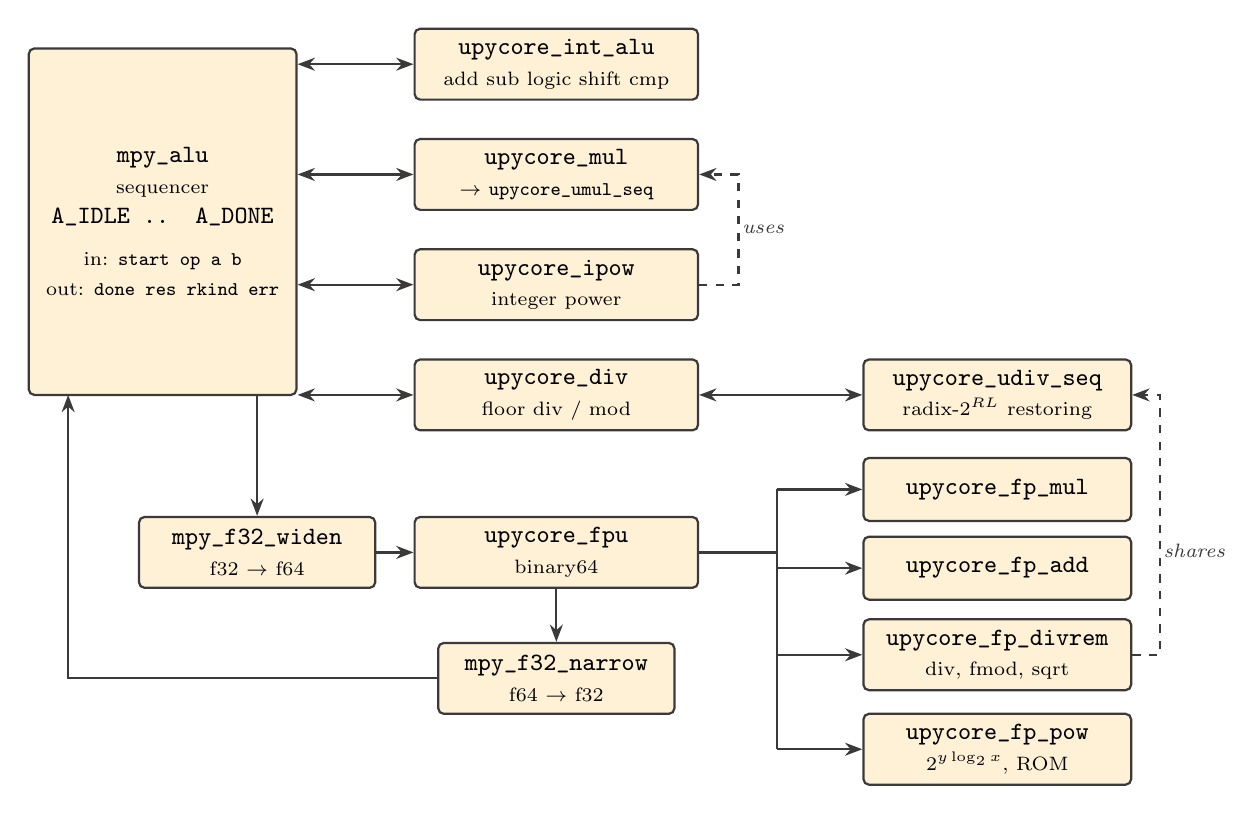
\begin{tikzpicture}
  \B{hw}{3.4}{4.4}{alu}{2.6,5.4}{\textbf{\rtl{mpy_alu}}\\\scriptsize sequencer\\\rtl{A_IDLE .. A_DONE}\\[4pt]\scriptsize in: \rtl{start op a b}\\\scriptsize out: \rtl{done res rkind err}}

  \B{hw}{3.6}{0.9}{int}{7.6,7.4}{\rtl{upycore_int_alu}\\\scriptsize add sub logic shift cmp}
  \B{hw}{3.6}{0.9}{mul}{7.6,6.0}{\rtl{upycore_mul}\\\scriptsize $\to$ \rtl{upycore_umul_seq}}
  \B{hw}{3.6}{0.9}{ipow}{7.6,4.6}{\rtl{upycore_ipow}\\\scriptsize integer power}
  \B{hw}{3.6}{0.9}{div}{7.6,3.2}{\rtl{upycore_div}\\\scriptsize floor div / mod}
  \B{hw}{3.6}{0.9}{fpu}{7.6,1.2}{\rtl{upycore_fpu}\\\scriptsize binary64}

  \B{hw}{3.4}{0.9}{udiv}{13.2,3.2}{\rtl{upycore_udiv_seq}\\\scriptsize radix-$2^{RL}$ restoring}
  \B{hw}{3.4}{0.8}{fmul}{13.2,2.0}{\rtl{upycore_fp_mul}}
  \B{hw}{3.4}{0.8}{fadd}{13.2,1.0}{\rtl{upycore_fp_add}}
  \B{hw}{3.4}{0.9}{fdiv}{13.2,-0.1}{\rtl{upycore_fp_divrem}\\\scriptsize div, fmod, sqrt}
  \B{hw}{3.4}{0.9}{fpow}{13.2,-1.3}{\rtl{upycore_fp_pow}\\\scriptsize $2^{y\log_2 x}$, ROM}

  \B{hw}{3.0}{0.9}{wid}{3.8,1.2}{\rtl{mpy_f32_widen}\\\scriptsize f32 $\to$ f64}
  \B{hw}{3.0}{0.9}{nar}{7.6,-0.4}{\rtl{mpy_f32_narrow}\\\scriptsize f64 $\to$ f32}

  \foreach \n in {int,mul,ipow,div} \draw[bbus] (alu.east |- \n.west) -- (\n.west);
  \draw[dbus] (ipow.east) -- ++(0.5,0) |- node[lab, pos=0.25, right] {uses} (mul.east);
  \draw[bbus] (div.east) -- (udiv.west);

  \draw[bus] (3.8,3.2) -- (wid.north);
  \draw[bus] (wid.east) -- (fpu.west);
  \draw[bus] (fpu.south) -- (nar.north);
  \draw[bus] (nar.west) -| (1.4,3.2);

  \draw[line] (fpu.east) -- (10.4,1.2);
  \draw[line] (10.4,2.0) -- (10.4,-1.3);
  \foreach \n/\y in {fmul/2.0,fadd/1.0,fdiv/-0.1,fpow/-1.3} \draw[bus] (10.4,\y) -- (\n.west);
  \draw[dbus] (fdiv.east) -- ++(0.35,0) |- node[lab, pos=0.2, right] {shares} (udiv.east);
\end{tikzpicture}
\caption{Arithmetic hierarchy. The integer unit is combinational; multiply,
divide, and power are sequenced; the FPU composes add / mul / div-rem / pow
pipelines into every float operation, with widen and narrow stages at the
ALU boundary.}
\label{fig:alu}
\end{figure}

% =============================================================================
\section{Garbage collector}
% =============================================================================

The pool is divided into 16-byte blocks tracked by a two-bit allocation table
(\rtl{FREE}, \rtl{HEAD}, \rtl{TAIL}, \rtl{MARK}). Allocation is next-fit with
zeroing. A collection marks from two root ranges, scans objects from an
explicit stack, and sweeps. On a mark-stack overflow, the stack drains, every
marked block is rescanned, and the loop repeats until a pass is overflow-free.

\begin{figure}[!htbp]
\centering
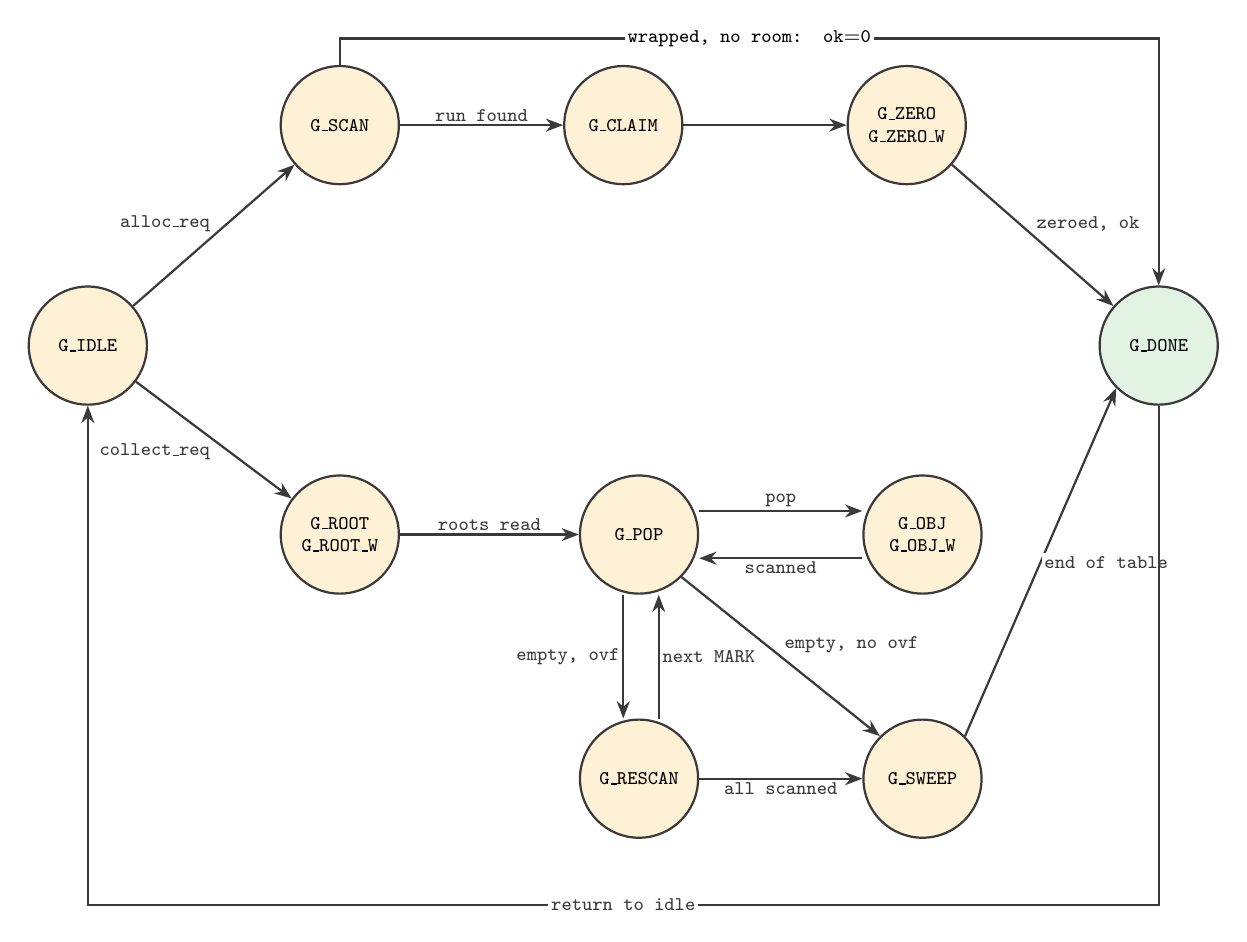
\begin{tikzpicture}
  \node[st] (idle)  at (1.0,3.8) {G\_IDLE};
  \node[st] (scan)  at (4.2,6.6) {G\_SCAN};
  \node[st] (claim) at (7.8,6.6) {G\_CLAIM};
  \node[st] (zero)  at (11.4,6.6) {G\_ZERO\\G\_ZERO\_W};
  \node[st,fill=cFW] (done) at (14.6,3.8) {G\_DONE};
  \node[st] (root)  at (4.2,1.4) {G\_ROOT\\G\_ROOT\_W};
  \node[st] (pop)   at (8.0,1.4) {G\_POP};
  \node[st] (obj)   at (11.6,1.4) {G\_OBJ\\G\_OBJ\_W};
  \node[st] (resc)  at (8.0,-1.7) {G\_RESCAN};
  \node[st] (sweep) at (11.6,-1.7) {G\_SWEEP};

  \draw[bus] (idle) -- node[sig, above left] {alloc\_req} (scan);
  \draw[bus] (scan) -- node[sig, above] {run found} (claim);
  \draw[bus] (claim) -- (zero);
  \draw[bus] (zero) -- node[sig, above right] {zeroed, ok} (done);
  \draw[bus] (scan.north) -- (4.2,7.7) -- (14.6,7.7) -- (done.north);
  \node[sig] at (9.4,7.7) {wrapped, no room: ok$=$0};

  \draw[bus] (idle) -- node[sig, below left] {collect\_req} (root);
  \draw[bus] (root) -- node[sig, above] {roots read} (pop);
  \draw[bus] ([yshift=0.3cm]pop.east) -- node[sig, above] {pop} ([yshift=0.3cm]obj.west);
  \draw[bus] ([yshift=-0.3cm]obj.west) -- node[sig, below] {scanned} ([yshift=-0.3cm]pop.east);
  \draw[bus] ([xshift=-0.2cm]pop.south) -- node[sig, left] {empty, ovf} ([xshift=-0.2cm]resc.north);
  \draw[bus] ([xshift=0.25cm]resc.north) -- node[sig, right] {next MARK} ([xshift=0.25cm]pop.south);
  \draw[bus] (pop.south east) -- node[sig, pos=0.5, above right] {empty, no ovf} (sweep.north west);
  \draw[bus] (resc) -- node[sig, below] {all scanned} (sweep);
  \draw[bus] (sweep.north east) -- node[sig, right, pos=0.5] {end of table} (done.south west);

  \draw[bus] (done.south) -- (14.6,-3.3) -- node[sig] {return to idle} (1.0,-3.3) -- (idle.south);
\end{tikzpicture}
\caption{\rtl{mpy_gc} state machine. Top row: allocation. Lower rows:
mark-sweep collection. State names follow the RTL \rtl{gstate_e} enum.}
\label{fig:gc}
\end{figure}

\begin{figure}[!htbp]
\centering
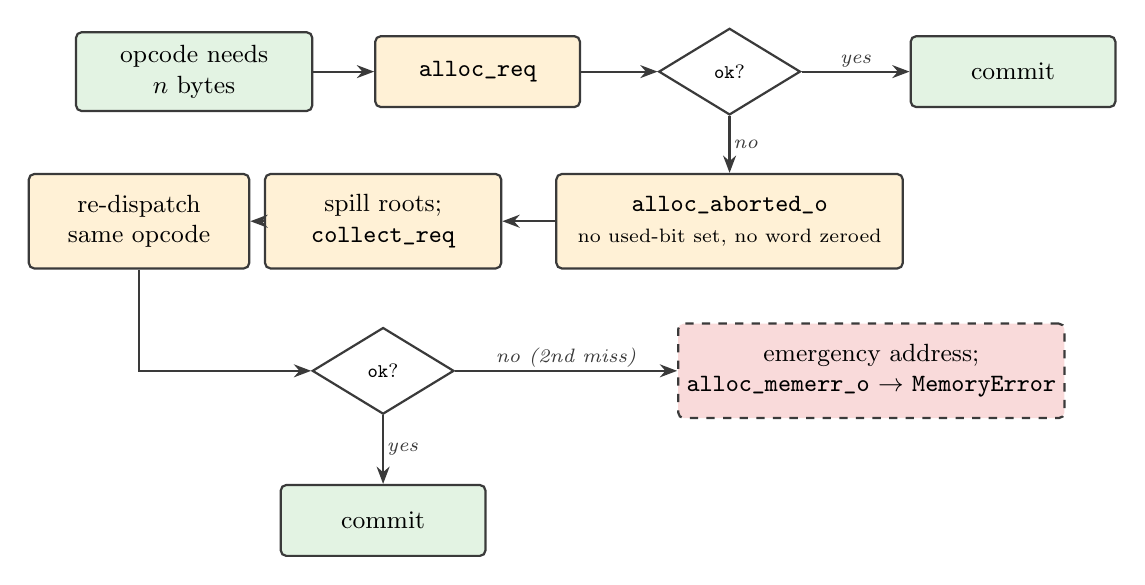
\begin{tikzpicture}
  \B{fw}{3.0}{1.0}{op}{1.6,4.0}{opcode needs\\$n$ bytes}
  \B{hw}{2.6}{0.9}{a1}{5.2,4.0}{\rtl{alloc_req}}
  \node[dec, minimum width=1.8cm, minimum height=1.1cm] (ok1) at (8.4,4.0) {\rtl{ok}?};
  \B{fw}{2.6}{0.9}{c1}{12.0,4.0}{commit}

  \B{hw}{4.4}{1.2}{abort}{8.4,2.1}{\rtl{alloc_aborted_o}\\\scriptsize no used-bit set, no word zeroed}
  \B{hw}{3.0}{1.2}{coll}{4.0,2.1}{spill roots;\\\rtl{collect_req}}
  \B{hw}{2.8}{1.2}{redo}{0.9,2.1}{re-dispatch\\same opcode}
  \node[dec, minimum width=1.8cm, minimum height=1.1cm] (ok2) at (4.0,0.2) {\rtl{ok}?};
  \B{todo}{4.4}{1.2}{me}{10.2,0.2}{emergency address;\\\rtl{alloc_memerr_o} $\to$ \rtl{MemoryError}}
  \B{fw}{2.6}{0.9}{c2}{4.0,-1.7}{commit}

  \draw[bus] (op) -- (a1);
  \draw[bus] (a1) -- (ok1);
  \draw[bus] (ok1) -- node[lab, above] {yes} (c1);
  \draw[bus] (ok1) -- node[lab, right] {no} (abort);
  \draw[bus] (abort) -- (coll);
  \draw[bus] (coll) -- (redo);
  \draw[bus] (redo.south) |- (ok2.west);
  \draw[bus] (ok2.south) -- node[lab, right] {yes} (c2.north);
  \draw[bus] (ok2.east) -- node[lab, above] {no (2nd miss)} (me.west);
\end{tikzpicture}
\caption{Allocation-failure protocol between \rtl{mpy_core} and \rtl{mpy_gc}.
The opcode aborts \emph{before} its first architectural commit, so the
re-dispatch after collection is exact. The second \rtl{alloc_req} reuses the
same size; its miss returns the pre-allocated emergency object.}
\label{fig:oom}
\end{figure}

% =============================================================================
\section{Interrupts and peripherals}
% =============================================================================

\rtl{mpy_periph} and \rtl{mpy_irq} implement the v1 MMIO register model
(\rtl{mpy_peripherals.md}). They have a standalone testbench and an
executable Python model (\rtl{mpy_periph_model.py}) but are \emph{not yet
instantiated} by \rtl{mpy_soc}; the hart will drive \rtl{bc_boundary} and
\rtl{jump} pulses and map stores in the handler-table range to
\rtl{handler_we}.

\begin{figure}[!htbp]
\centering
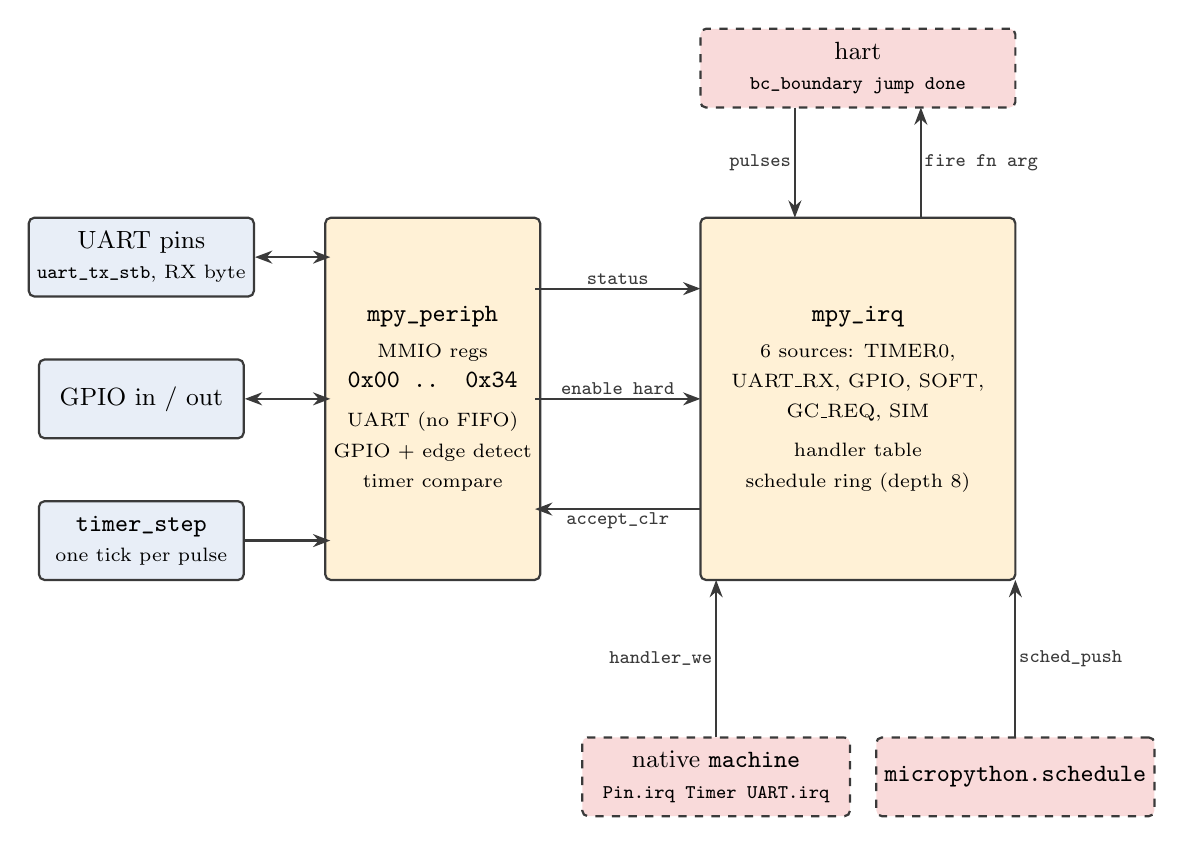
\begin{tikzpicture}
  \B{host}{2.6}{1.0}{uart}{1.3,5.6}{UART pins\\\scriptsize\rtl{uart_tx_stb}, RX byte}
  \B{host}{2.6}{1.0}{gpio}{1.3,3.8}{GPIO in / out}
  \B{host}{2.6}{1.0}{tick}{1.3,2.0}{\rtl{timer_step}\\\scriptsize one tick per pulse}

  \B{hw}{2.6}{4.6}{per}{5.0,3.8}{\textbf{\rtl{mpy_periph}}\\[2pt]\scriptsize MMIO regs\\\rtl{0x00 .. 0x34}\\[3pt]\scriptsize UART (no FIFO)\\\scriptsize GPIO + edge detect\\\scriptsize timer compare}
  \B{hw}{4.0}{4.6}{irq}{10.4,3.8}{\textbf{\rtl{mpy_irq}}\\[2pt]\scriptsize 6 sources: TIMER0,\\\scriptsize UART\_RX, GPIO, SOFT,\\\scriptsize GC\_REQ, SIM\\[3pt]\scriptsize handler table\\\scriptsize schedule ring (depth 8)}

  \B{todo}{4.0}{1.0}{hart}{10.4,8.0}{hart\\\scriptsize\rtl{bc_boundary jump done}}
  \B{todo}{3.4}{1.0}{mach}{8.6,-1.0}{native \rtl{machine}\\\scriptsize\rtl{Pin.irq Timer UART.irq}}
  \B{todo}{3.4}{1.0}{sched}{12.4,-1.0}{\rtl{micropython.schedule}}

  \draw[bbus] (uart.east) -- (3.7,5.6);
  \draw[bbus] (gpio.east) -- (3.7,3.8);
  \draw[bus]  (tick.east) -- (3.7,2.0);

  \draw[bus] (6.3,5.2) -- node[sig, above] {\rtl{status}} (8.4,5.2);
  \draw[bus] (6.3,3.8) -- node[sig, above] {\rtl{enable hard}} (8.4,3.8);
  \draw[bus] (8.4,2.4) -- node[sig, below] {\rtl{accept_clr}} (6.3,2.4);

  \draw[bus] (9.6,7.5) -- node[sig, left] {\rtl{pulses}} (9.6,6.1);
  \draw[bus] (11.2,6.1) -- node[sig, right] {\rtl{fire fn arg}} (11.2,7.5);
  \draw[bus] (8.6,-0.5) -- node[sig, left] {\rtl{handler_we}} (8.6,1.5);
  \draw[bus] (12.4,-0.5) -- node[sig, right] {\rtl{sched_push}} (12.4,1.5);
\end{tikzpicture}
\caption{Peripheral and interrupt block. Red dashed blocks are the intended
hart-side and software consumers; they are not connected in the current tree.}
\label{fig:irq}
\end{figure}

\begin{figure}[!htbp]
\centering
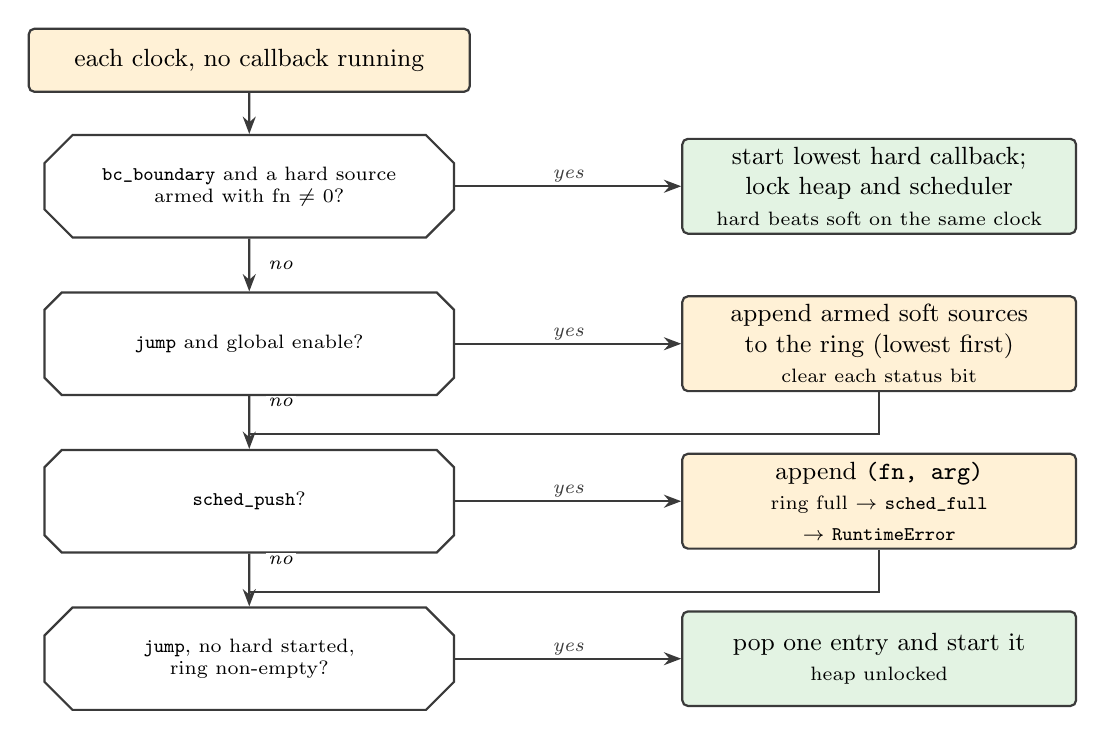
\begin{tikzpicture}
  \B{hw}{5.6}{0.8}{clk}{3.2,8.2}{each clock, no callback running}
  \node[cond, minimum width=5.2cm, minimum height=1.3cm] (hard) at (3.2,6.6) {\rtl{bc_boundary} and a hard source\\armed with fn $\ne$ 0?};
  \node[cond, minimum width=5.2cm, minimum height=1.3cm] (soft) at (3.2,4.6) {\rtl{jump} and global enable?};
  \node[cond, minimum width=5.2cm, minimum height=1.3cm] (push) at (3.2,2.6) {\rtl{sched_push}?};
  \node[cond, minimum width=5.2cm, minimum height=1.3cm] (pop)  at (3.2,0.6) {\rtl{jump}, no hard started,\\ring non-empty?};

  \B{fw}{5.0}{1.2}{fh}{11.2,6.6}{start lowest hard callback;\\lock heap and scheduler\\\scriptsize hard beats soft on the same clock}
  \B{hw}{5.0}{1.2}{q1}{11.2,4.6}{append armed soft sources\\to the ring (lowest first)\\\scriptsize clear each status bit}
  \B{hw}{5.0}{1.2}{q2}{11.2,2.6}{append \rtl{(fn, arg)}\\\scriptsize ring full $\to$ \rtl{sched_full}\\\scriptsize $\to$ \rtl{RuntimeError}}
  \B{fw}{5.0}{1.2}{run}{11.2,0.6}{pop one entry and start it\\\scriptsize heap unlocked}

  \draw[bus] (clk) -- (hard);
  \draw[bus] (hard) -- (soft);  \node[lab] at (3.6,5.6) {no};
  \draw[bus] (soft) -- (push);  \node[lab] at (3.6,3.85) {no};
  \draw[bus] (push) -- (pop);   \node[lab] at (3.6,1.85) {no};
  \draw[bus] (hard.east) -- node[lab, above] {yes} (fh.west);
  \draw[bus] (soft.east) -- node[lab, above] {yes} (q1.west);
  \draw[bus] (push.east) -- node[lab, above] {yes} (q2.west);
  \draw[bus] (pop.east) -- node[lab, above] {yes} (run.west);
  \draw[line] (q1.south) -- (11.2,3.45) -- (3.2,3.45);
  \draw[line] (q2.south) -- (11.2,1.45) -- (3.2,1.45);
\end{tikzpicture}
\caption{Per-clock callback selection in \rtl{mpy_irq}, in priority order. Soft
device IRQs and \rtl{micropython.schedule} share one ring and run one callback
at a jump opcode. A callback that was queued on an empty ring runs on that
same jump. There is no nesting.}
\label{fig:irqorder}
\end{figure}

% =============================================================================
\section{Verification map}
% =============================================================================

\begin{figure}[!htbp]
\centering
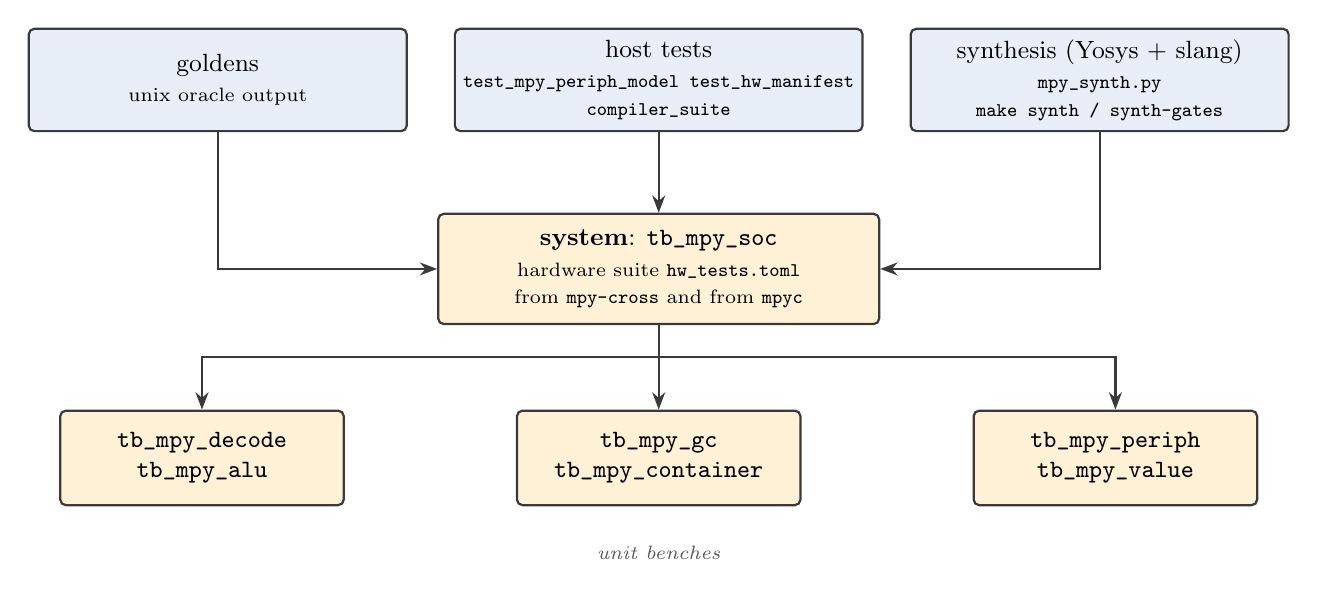
\begin{tikzpicture}
  \B{host}{4.8}{1.3}{gold}{2.6,5.0}{goldens\\\scriptsize unix oracle output}
  \B{host}{4.8}{1.3}{host}{8.2,5.0}{host tests\\\scriptsize\rtl{test_mpy_periph_model test_hw_manifest}\\[-1pt]\scriptsize\rtl{compiler_suite}}
  \B{host}{4.8}{1.3}{syn}{13.8,5.0}{synthesis (Yosys + slang)\\\scriptsize\rtl{mpy_synth.py}\\[-1pt]\scriptsize\rtl{make synth / synth-gates}}

  \B{hw}{5.6}{1.4}{soc}{8.2,2.6}{\textbf{system}: \rtl{tb_mpy_soc}\\\scriptsize hardware suite \rtl{hw_tests.toml}\\[-1pt]\scriptsize from \rtl{mpy-cross} and from \rtl{mpyc}}
  \B{hw}{3.6}{1.2}{u1}{2.4,0.2}{\rtl{tb_mpy_decode}\\\rtl{tb_mpy_alu}}
  \B{hw}{3.6}{1.2}{u2}{8.2,0.2}{\rtl{tb_mpy_gc}\\\rtl{tb_mpy_container}}
  \B{hw}{3.6}{1.2}{u3}{14.0,0.2}{\rtl{tb_mpy_periph}\\\rtl{tb_mpy_value}}

  \draw[bus] (gold.south) |- (soc.west);
  \draw[bus] (host.south) -- (soc.north);
  \draw[bus] (syn.south) |- (soc.east);
  \draw[bus] (soc.south) -- ++(0,-0.4) -| (u1.north);
  \draw[bus] (soc.south) -- (u2.north);
  \draw[bus] (soc.south) -- ++(0,-0.4) -| (u3.north);
  \node[note] at (8.2,-1.0) {unit benches};
\end{tikzpicture}
\caption{Test layering. System-level runs compare stdout, stderr, and exit
status with the oracle's golden files, from both compilers; unit benches
exercise the decoder, ALU, collector, container engine, and peripheral block
in isolation; a Yosys flow elaborates every top and gate-maps the logic tops.}
\label{fig:verif}
\end{figure}

\end{document}
